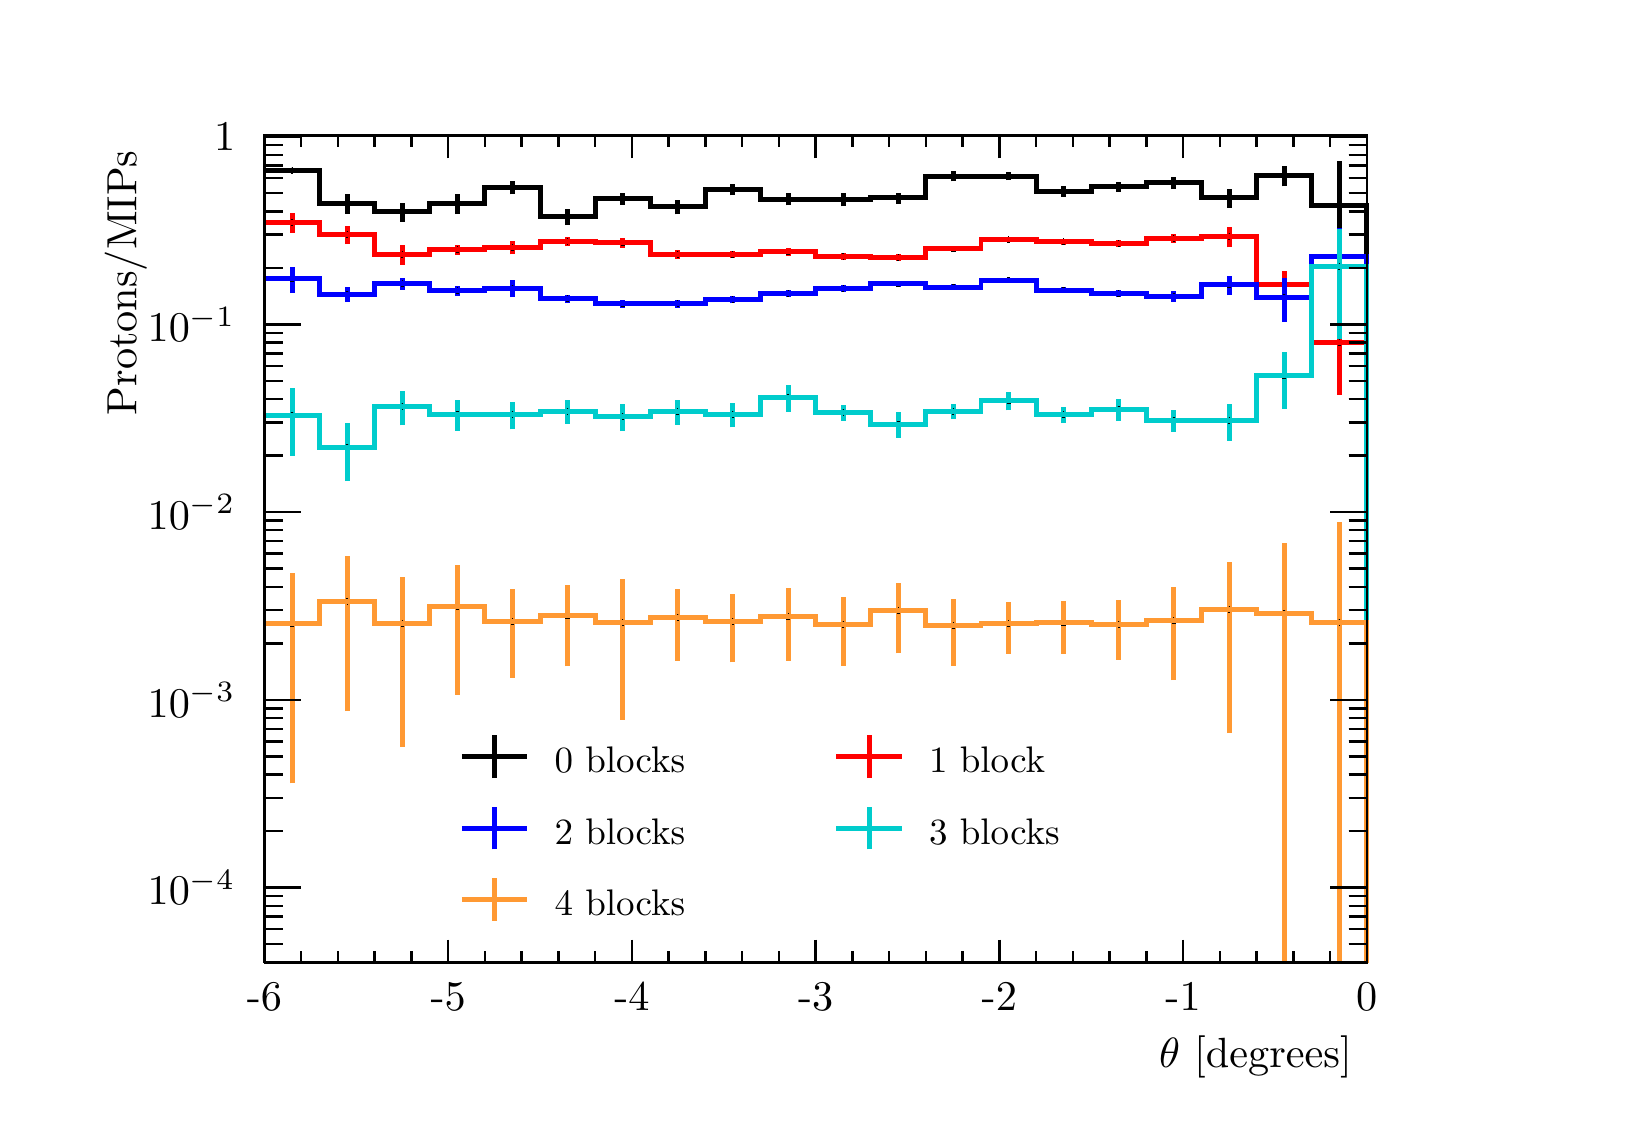
\begin{tikzpicture}
\pgfdeclareplotmark{cross} {
\pgfpathmoveto{\pgfpoint{-0.3\pgfplotmarksize}{\pgfplotmarksize}}
\pgfpathlineto{\pgfpoint{+0.3\pgfplotmarksize}{\pgfplotmarksize}}
\pgfpathlineto{\pgfpoint{+0.3\pgfplotmarksize}{0.3\pgfplotmarksize}}
\pgfpathlineto{\pgfpoint{+1\pgfplotmarksize}{0.3\pgfplotmarksize}}
\pgfpathlineto{\pgfpoint{+1\pgfplotmarksize}{-0.3\pgfplotmarksize}}
\pgfpathlineto{\pgfpoint{+0.3\pgfplotmarksize}{-0.3\pgfplotmarksize}}
\pgfpathlineto{\pgfpoint{+0.3\pgfplotmarksize}{-1.\pgfplotmarksize}}
\pgfpathlineto{\pgfpoint{-0.3\pgfplotmarksize}{-1.\pgfplotmarksize}}
\pgfpathlineto{\pgfpoint{-0.3\pgfplotmarksize}{-0.3\pgfplotmarksize}}
\pgfpathlineto{\pgfpoint{-1.\pgfplotmarksize}{-0.3\pgfplotmarksize}}
\pgfpathlineto{\pgfpoint{-1.\pgfplotmarksize}{0.3\pgfplotmarksize}}
\pgfpathlineto{\pgfpoint{-0.3\pgfplotmarksize}{0.3\pgfplotmarksize}}
\pgfpathclose
\pgfusepathqstroke
}
\pgfdeclareplotmark{cross*} {
\pgfpathmoveto{\pgfpoint{-0.3\pgfplotmarksize}{\pgfplotmarksize}}
\pgfpathlineto{\pgfpoint{+0.3\pgfplotmarksize}{\pgfplotmarksize}}
\pgfpathlineto{\pgfpoint{+0.3\pgfplotmarksize}{0.3\pgfplotmarksize}}
\pgfpathlineto{\pgfpoint{+1\pgfplotmarksize}{0.3\pgfplotmarksize}}
\pgfpathlineto{\pgfpoint{+1\pgfplotmarksize}{-0.3\pgfplotmarksize}}
\pgfpathlineto{\pgfpoint{+0.3\pgfplotmarksize}{-0.3\pgfplotmarksize}}
\pgfpathlineto{\pgfpoint{+0.3\pgfplotmarksize}{-1.\pgfplotmarksize}}
\pgfpathlineto{\pgfpoint{-0.3\pgfplotmarksize}{-1.\pgfplotmarksize}}
\pgfpathlineto{\pgfpoint{-0.3\pgfplotmarksize}{-0.3\pgfplotmarksize}}
\pgfpathlineto{\pgfpoint{-1.\pgfplotmarksize}{-0.3\pgfplotmarksize}}
\pgfpathlineto{\pgfpoint{-1.\pgfplotmarksize}{0.3\pgfplotmarksize}}
\pgfpathlineto{\pgfpoint{-0.3\pgfplotmarksize}{0.3\pgfplotmarksize}}
\pgfpathclose
\pgfusepathqfillstroke
}
\pgfdeclareplotmark{newstar} {
\pgfpathmoveto{\pgfqpoint{0pt}{\pgfplotmarksize}}
\pgfpathlineto{\pgfqpointpolar{44}{0.5\pgfplotmarksize}}
\pgfpathlineto{\pgfqpointpolar{18}{\pgfplotmarksize}}
\pgfpathlineto{\pgfqpointpolar{-20}{0.5\pgfplotmarksize}}
\pgfpathlineto{\pgfqpointpolar{-54}{\pgfplotmarksize}}
\pgfpathlineto{\pgfqpointpolar{-90}{0.5\pgfplotmarksize}}
\pgfpathlineto{\pgfqpointpolar{234}{\pgfplotmarksize}}
\pgfpathlineto{\pgfqpointpolar{198}{0.5\pgfplotmarksize}}
\pgfpathlineto{\pgfqpointpolar{162}{\pgfplotmarksize}}
\pgfpathlineto{\pgfqpointpolar{134}{0.5\pgfplotmarksize}}
\pgfpathclose
\pgfusepathqstroke
}
\pgfdeclareplotmark{newstar*} {
\pgfpathmoveto{\pgfqpoint{0pt}{\pgfplotmarksize}}
\pgfpathlineto{\pgfqpointpolar{44}{0.5\pgfplotmarksize}}
\pgfpathlineto{\pgfqpointpolar{18}{\pgfplotmarksize}}
\pgfpathlineto{\pgfqpointpolar{-20}{0.5\pgfplotmarksize}}
\pgfpathlineto{\pgfqpointpolar{-54}{\pgfplotmarksize}}
\pgfpathlineto{\pgfqpointpolar{-90}{0.5\pgfplotmarksize}}
\pgfpathlineto{\pgfqpointpolar{234}{\pgfplotmarksize}}
\pgfpathlineto{\pgfqpointpolar{198}{0.5\pgfplotmarksize}}
\pgfpathlineto{\pgfqpointpolar{162}{\pgfplotmarksize}}
\pgfpathlineto{\pgfqpointpolar{134}{0.5\pgfplotmarksize}}
\pgfpathclose
\pgfusepathqfillstroke
}
\definecolor{c}{rgb}{1,1,1};
\draw [color=c, fill=c] (0,0) rectangle (20,13.639);
\draw [color=c, fill=c] (3,1.77307) rectangle (17,12.2751);
\definecolor{c}{rgb}{0,0,0};
\draw [c,line width=0.9] (3,1.77307) -- (3,12.2751) -- (17,12.2751) -- (17,1.77307) -- (3,1.77307);
\definecolor{c}{rgb}{1,1,1};
\draw [color=c, fill=c] (3,1.77307) rectangle (17,12.2751);
\definecolor{c}{rgb}{0,0,0};
\draw [c,line width=0.9] (3,1.77307) -- (3,12.2751) -- (17,12.2751) -- (17,1.77307) -- (3,1.77307);
\draw [c,line width=0.9] (3,1.77307) -- (3.7,1.77307) -- (3.7,1.77307) -- (4.4,1.77307) -- (4.4,1.77307) -- (5.1,1.77307) -- (5.1,1.77307) -- (5.8,1.77307) -- (5.8,1.77307) -- (6.5,1.77307) -- (6.5,1.77307) -- (7.2,1.77307) -- (7.2,1.77307) --
 (7.9,1.77307) -- (7.9,1.77307) -- (8.6,1.77307) -- (8.6,1.77307) -- (9.3,1.77307) -- (9.3,1.77307) -- (10,1.77307) -- (10,1.77307) -- (10.7,1.77307) -- (10.7,1.77307) -- (11.4,1.77307) -- (11.4,1.77307) -- (12.1,1.77307) -- (12.1,1.77307) --
 (12.8,1.77307) -- (12.8,1.77307) -- (13.5,1.77307) -- (13.5,1.77307) -- (14.2,1.77307) -- (14.2,1.77307) -- (14.9,1.77307) -- (14.9,1.77307) -- (15.6,1.77307) -- (15.6,1.77307) -- (16.3,1.77307) -- (16.3,1.77307) -- (17,1.77307) -- (17,1.77307);
\draw [c,line width=0.9] (3,1.77307) -- (17,1.77307);
\draw [c,line width=0.9] (3,2.05948) -- (3,1.77307);
\draw [c,line width=0.9] (3.46667,1.91628) -- (3.46667,1.77307);
\draw [c,line width=0.9] (3.93333,1.91628) -- (3.93333,1.77307);
\draw [c,line width=0.9] (4.4,1.91628) -- (4.4,1.77307);
\draw [c,line width=0.9] (4.86667,1.91628) -- (4.86667,1.77307);
\draw [c,line width=0.9] (5.33333,2.05948) -- (5.33333,1.77307);
\draw [c,line width=0.9] (5.8,1.91628) -- (5.8,1.77307);
\draw [c,line width=0.9] (6.26667,1.91628) -- (6.26667,1.77307);
\draw [c,line width=0.9] (6.73333,1.91628) -- (6.73333,1.77307);
\draw [c,line width=0.9] (7.2,1.91628) -- (7.2,1.77307);
\draw [c,line width=0.9] (7.66667,2.05948) -- (7.66667,1.77307);
\draw [c,line width=0.9] (8.13333,1.91628) -- (8.13333,1.77307);
\draw [c,line width=0.9] (8.6,1.91628) -- (8.6,1.77307);
\draw [c,line width=0.9] (9.06667,1.91628) -- (9.06667,1.77307);
\draw [c,line width=0.9] (9.53333,1.91628) -- (9.53333,1.77307);
\draw [c,line width=0.9] (10,2.05948) -- (10,1.77307);
\draw [c,line width=0.9] (10.4667,1.91628) -- (10.4667,1.77307);
\draw [c,line width=0.9] (10.9333,1.91628) -- (10.9333,1.77307);
\draw [c,line width=0.9] (11.4,1.91628) -- (11.4,1.77307);
\draw [c,line width=0.9] (11.8667,1.91628) -- (11.8667,1.77307);
\draw [c,line width=0.9] (12.3333,2.05948) -- (12.3333,1.77307);
\draw [c,line width=0.9] (12.8,1.91628) -- (12.8,1.77307);
\draw [c,line width=0.9] (13.2667,1.91628) -- (13.2667,1.77307);
\draw [c,line width=0.9] (13.7333,1.91628) -- (13.7333,1.77307);
\draw [c,line width=0.9] (14.2,1.91628) -- (14.2,1.77307);
\draw [c,line width=0.9] (14.6667,2.05948) -- (14.6667,1.77307);
\draw [c,line width=0.9] (15.1333,1.91628) -- (15.1333,1.77307);
\draw [c,line width=0.9] (15.6,1.91628) -- (15.6,1.77307);
\draw [c,line width=0.9] (16.0667,1.91628) -- (16.0667,1.77307);
\draw [c,line width=0.9] (16.5333,1.91628) -- (16.5333,1.77307);
\draw [c,line width=0.9] (17,2.05948) -- (17,1.77307);
\draw [anchor=base] (3,1.15931) node[scale=1.52731, color=c, rotate=0]{-6};
\draw [anchor=base] (5.33333,1.15931) node[scale=1.52731, color=c, rotate=0]{-5};
\draw [anchor=base] (7.66667,1.15931) node[scale=1.52731, color=c, rotate=0]{-4};
\draw [anchor=base] (10,1.15931) node[scale=1.52731, color=c, rotate=0]{-3};
\draw [anchor=base] (12.3333,1.15931) node[scale=1.52731, color=c, rotate=0]{-2};
\draw [anchor=base] (14.6667,1.15931) node[scale=1.52731, color=c, rotate=0]{-1};
\draw [anchor=base] (17,1.15931) node[scale=1.52731, color=c, rotate=0]{0};
\draw [anchor= east] (17,0.572837) node[scale=1.52731, color=c, rotate=0]{$\theta$ [degrees] };
\draw [c,line width=0.9] (3,12.2751) -- (17,12.2751);
\draw [c,line width=0.9] (3,11.9887) -- (3,12.2751);
\draw [c,line width=0.9] (3.46667,12.1319) -- (3.46667,12.2751);
\draw [c,line width=0.9] (3.93333,12.1319) -- (3.93333,12.2751);
\draw [c,line width=0.9] (4.4,12.1319) -- (4.4,12.2751);
\draw [c,line width=0.9] (4.86667,12.1319) -- (4.86667,12.2751);
\draw [c,line width=0.9] (5.33333,11.9887) -- (5.33333,12.2751);
\draw [c,line width=0.9] (5.8,12.1319) -- (5.8,12.2751);
\draw [c,line width=0.9] (6.26667,12.1319) -- (6.26667,12.2751);
\draw [c,line width=0.9] (6.73333,12.1319) -- (6.73333,12.2751);
\draw [c,line width=0.9] (7.2,12.1319) -- (7.2,12.2751);
\draw [c,line width=0.9] (7.66667,11.9887) -- (7.66667,12.2751);
\draw [c,line width=0.9] (8.13333,12.1319) -- (8.13333,12.2751);
\draw [c,line width=0.9] (8.6,12.1319) -- (8.6,12.2751);
\draw [c,line width=0.9] (9.06667,12.1319) -- (9.06667,12.2751);
\draw [c,line width=0.9] (9.53333,12.1319) -- (9.53333,12.2751);
\draw [c,line width=0.9] (10,11.9887) -- (10,12.2751);
\draw [c,line width=0.9] (10.4667,12.1319) -- (10.4667,12.2751);
\draw [c,line width=0.9] (10.9333,12.1319) -- (10.9333,12.2751);
\draw [c,line width=0.9] (11.4,12.1319) -- (11.4,12.2751);
\draw [c,line width=0.9] (11.8667,12.1319) -- (11.8667,12.2751);
\draw [c,line width=0.9] (12.3333,11.9887) -- (12.3333,12.2751);
\draw [c,line width=0.9] (12.8,12.1319) -- (12.8,12.2751);
\draw [c,line width=0.9] (13.2667,12.1319) -- (13.2667,12.2751);
\draw [c,line width=0.9] (13.7333,12.1319) -- (13.7333,12.2751);
\draw [c,line width=0.9] (14.2,12.1319) -- (14.2,12.2751);
\draw [c,line width=0.9] (14.6667,11.9887) -- (14.6667,12.2751);
\draw [c,line width=0.9] (15.1333,12.1319) -- (15.1333,12.2751);
\draw [c,line width=0.9] (15.6,12.1319) -- (15.6,12.2751);
\draw [c,line width=0.9] (16.0667,12.1319) -- (16.0667,12.2751);
\draw [c,line width=0.9] (16.5333,12.1319) -- (16.5333,12.2751);
\draw [c,line width=0.9] (17,11.9887) -- (17,12.2751);
\draw [c,line width=0.9] (3,1.77307) -- (3,12.2751);
\draw [c,line width=0.9] (3.231,1.77653) -- (3,1.77653);
\draw [c,line width=0.9] (3.231,2.0076) -- (3,2.0076);
\draw [c,line width=0.9] (3.231,2.1964) -- (3,2.1964);
\draw [c,line width=0.9] (3.231,2.35603) -- (3,2.35603);
\draw [c,line width=0.9] (3.231,2.49431) -- (3,2.49431);
\draw [c,line width=0.9] (3.231,2.61628) -- (3,2.61628);
\draw [c,line width=0.9] (3.462,2.72539) -- (3,2.72539);
\draw [anchor= east] (2.82,2.72539) node[scale=1.52731, color=c, rotate=0]{$10^{-4}$};
\draw [c,line width=0.9] (3.231,3.44317) -- (3,3.44317);
\draw [c,line width=0.9] (3.231,3.86305) -- (3,3.86305);
\draw [c,line width=0.9] (3.231,4.16096) -- (3,4.16096);
\draw [c,line width=0.9] (3.231,4.39203) -- (3,4.39203);
\draw [c,line width=0.9] (3.231,4.58083) -- (3,4.58083);
\draw [c,line width=0.9] (3.231,4.74046) -- (3,4.74046);
\draw [c,line width=0.9] (3.231,4.87874) -- (3,4.87874);
\draw [c,line width=0.9] (3.231,5.00071) -- (3,5.00071);
\draw [c,line width=0.9] (3.462,5.10982) -- (3,5.10982);
\draw [anchor= east] (2.82,5.10982) node[scale=1.52731, color=c, rotate=0]{$10^{-3}$};
\draw [c,line width=0.9] (3.231,5.8276) -- (3,5.8276);
\draw [c,line width=0.9] (3.231,6.24748) -- (3,6.24748);
\draw [c,line width=0.9] (3.231,6.54539) -- (3,6.54539);
\draw [c,line width=0.9] (3.231,6.77646) -- (3,6.77646);
\draw [c,line width=0.9] (3.231,6.96527) -- (3,6.96527);
\draw [c,line width=0.9] (3.231,7.1249) -- (3,7.1249);
\draw [c,line width=0.9] (3.231,7.26317) -- (3,7.26317);
\draw [c,line width=0.9] (3.231,7.38514) -- (3,7.38514);
\draw [c,line width=0.9] (3.462,7.49425) -- (3,7.49425);
\draw [anchor= east] (2.82,7.49425) node[scale=1.52731, color=c, rotate=0]{$10^{-2}$};
\draw [c,line width=0.9] (3.231,8.21203) -- (3,8.21203);
\draw [c,line width=0.9] (3.231,8.63191) -- (3,8.63191);
\draw [c,line width=0.9] (3.231,8.92982) -- (3,8.92982);
\draw [c,line width=0.9] (3.231,9.16089) -- (3,9.16089);
\draw [c,line width=0.9] (3.231,9.3497) -- (3,9.3497);
\draw [c,line width=0.9] (3.231,9.50933) -- (3,9.50933);
\draw [c,line width=0.9] (3.231,9.6476) -- (3,9.6476);
\draw [c,line width=0.9] (3.231,9.76957) -- (3,9.76957);
\draw [c,line width=0.9] (3.462,9.87868) -- (3,9.87868);
\draw [anchor= east] (2.82,9.87868) node[scale=1.52731, color=c, rotate=0]{$10^{-1}$};
\draw [c,line width=0.9] (3.231,10.5965) -- (3,10.5965);
\draw [c,line width=0.9] (3.231,11.0163) -- (3,11.0163);
\draw [c,line width=0.9] (3.231,11.3142) -- (3,11.3142);
\draw [c,line width=0.9] (3.231,11.5453) -- (3,11.5453);
\draw [c,line width=0.9] (3.231,11.7341) -- (3,11.7341);
\draw [c,line width=0.9] (3.231,11.8938) -- (3,11.8938);
\draw [c,line width=0.9] (3.231,12.032) -- (3,12.032);
\draw [c,line width=0.9] (3.231,12.154) -- (3,12.154);
\draw [c,line width=0.9] (3.462,12.2631) -- (3,12.2631);
\draw [anchor= east] (2.82,12.2631) node[scale=1.52731, color=c, rotate=0]{1};
\draw [anchor= east] (1.24,12.2751) node[scale=1.52731, color=c, rotate=90]{ Protons/MIPs};
\draw [c,line width=0.9] (17,1.77307) -- (17,12.2751);
\draw [c,line width=0.9] (16.769,1.77653) -- (17,1.77653);
\draw [c,line width=0.9] (16.769,2.0076) -- (17,2.0076);
\draw [c,line width=0.9] (16.769,2.1964) -- (17,2.1964);
\draw [c,line width=0.9] (16.769,2.35603) -- (17,2.35603);
\draw [c,line width=0.9] (16.769,2.49431) -- (17,2.49431);
\draw [c,line width=0.9] (16.769,2.61628) -- (17,2.61628);
\draw [c,line width=0.9] (16.538,2.72539) -- (17,2.72539);
\draw [c,line width=0.9] (16.769,3.44317) -- (17,3.44317);
\draw [c,line width=0.9] (16.769,3.86305) -- (17,3.86305);
\draw [c,line width=0.9] (16.769,4.16096) -- (17,4.16096);
\draw [c,line width=0.9] (16.769,4.39203) -- (17,4.39203);
\draw [c,line width=0.9] (16.769,4.58083) -- (17,4.58083);
\draw [c,line width=0.9] (16.769,4.74046) -- (17,4.74046);
\draw [c,line width=0.9] (16.769,4.87874) -- (17,4.87874);
\draw [c,line width=0.9] (16.769,5.00071) -- (17,5.00071);
\draw [c,line width=0.9] (16.538,5.10982) -- (17,5.10982);
\draw [c,line width=0.9] (16.769,5.8276) -- (17,5.8276);
\draw [c,line width=0.9] (16.769,6.24748) -- (17,6.24748);
\draw [c,line width=0.9] (16.769,6.54539) -- (17,6.54539);
\draw [c,line width=0.9] (16.769,6.77646) -- (17,6.77646);
\draw [c,line width=0.9] (16.769,6.96527) -- (17,6.96527);
\draw [c,line width=0.9] (16.769,7.1249) -- (17,7.1249);
\draw [c,line width=0.9] (16.769,7.26317) -- (17,7.26317);
\draw [c,line width=0.9] (16.769,7.38514) -- (17,7.38514);
\draw [c,line width=0.9] (16.538,7.49425) -- (17,7.49425);
\draw [c,line width=0.9] (16.769,8.21203) -- (17,8.21203);
\draw [c,line width=0.9] (16.769,8.63191) -- (17,8.63191);
\draw [c,line width=0.9] (16.769,8.92982) -- (17,8.92982);
\draw [c,line width=0.9] (16.769,9.16089) -- (17,9.16089);
\draw [c,line width=0.9] (16.769,9.3497) -- (17,9.3497);
\draw [c,line width=0.9] (16.769,9.50933) -- (17,9.50933);
\draw [c,line width=0.9] (16.769,9.6476) -- (17,9.6476);
\draw [c,line width=0.9] (16.769,9.76957) -- (17,9.76957);
\draw [c,line width=0.9] (16.538,9.87868) -- (17,9.87868);
\draw [c,line width=0.9] (16.769,10.5965) -- (17,10.5965);
\draw [c,line width=0.9] (16.769,11.0163) -- (17,11.0163);
\draw [c,line width=0.9] (16.769,11.3142) -- (17,11.3142);
\draw [c,line width=0.9] (16.769,11.5453) -- (17,11.5453);
\draw [c,line width=0.9] (16.769,11.7341) -- (17,11.7341);
\draw [c,line width=0.9] (16.769,11.8938) -- (17,11.8938);
\draw [c,line width=0.9] (16.769,12.032) -- (17,12.032);
\draw [c,line width=0.9] (16.769,12.154) -- (17,12.154);
\draw [c,line width=0.9] (16.538,12.2631) -- (17,12.2631);
\draw [c,line width=1.8] (3.35,11.7944) -- (3.35,11.8326);
\draw [c,line width=1.8] (3.35,11.8326) -- (3.35,11.8695);
\foreach \P in {(3.35,11.8326)}{\draw[mark options={color=c,fill=c},mark size=2.402402pt, line width=0.000000pt, mark=*,mark size=1pt] plot coordinates {\P};}
\draw [c,line width=1.8] (4.05,11.2801) -- (4.05,11.4121);
\draw [c,line width=1.8] (4.05,11.4121) -- (4.05,11.5292);
\foreach \P in {(4.05,11.4121)}{\draw[mark options={color=c,fill=c},mark size=2.402402pt, line width=0.000000pt, mark=*,mark size=1pt] plot coordinates {\P};}
\draw [c,line width=1.8] (4.75,11.1787) -- (4.75,11.3065);
\draw [c,line width=1.8] (4.75,11.3065) -- (4.75,11.4203);
\foreach \P in {(4.75,11.3065)}{\draw[mark options={color=c,fill=c},mark size=2.402402pt, line width=0.000000pt, mark=*,mark size=1pt] plot coordinates {\P};}
\draw [c,line width=1.8] (5.45,11.2778) -- (5.45,11.4122);
\draw [c,line width=1.8] (5.45,11.4122) -- (5.45,11.5311);
\foreach \P in {(5.45,11.4122)}{\draw[mark options={color=c,fill=c},mark size=2.402402pt, line width=0.000000pt, mark=*,mark size=1pt] plot coordinates {\P};}
\draw [c,line width=1.8] (6.15,11.5292) -- (6.15,11.617);
\draw [c,line width=1.8] (6.15,11.617) -- (6.15,11.6979);
\foreach \P in {(6.15,11.617)}{\draw[mark options={color=c,fill=c},mark size=2.402402pt, line width=0.000000pt, mark=*,mark size=1pt] plot coordinates {\P};}
\draw [c,line width=1.8] (6.85,11.1391) -- (6.85,11.2438);
\draw [c,line width=1.8] (6.85,11.2438) -- (6.85,11.3388);
\foreach \P in {(6.85,11.2438)}{\draw[mark options={color=c,fill=c},mark size=2.402402pt, line width=0.000000pt, mark=*,mark size=1pt] plot coordinates {\P};}
\draw [c,line width=1.8] (7.55,11.397) -- (7.55,11.4769);
\draw [c,line width=1.8] (7.55,11.4769) -- (7.55,11.551);
\foreach \P in {(7.55,11.4769)}{\draw[mark options={color=c,fill=c},mark size=2.402402pt, line width=0.000000pt, mark=*,mark size=1pt] plot coordinates {\P};}
\draw [c,line width=1.8] (8.25,11.2744) -- (8.25,11.3688);
\draw [c,line width=1.8] (8.25,11.3688) -- (8.25,11.4553);
\foreach \P in {(8.25,11.3688)}{\draw[mark options={color=c,fill=c},mark size=2.402402pt, line width=0.000000pt, mark=*,mark size=1pt] plot coordinates {\P};}
\draw [c,line width=1.8] (8.95,11.5168) -- (8.95,11.5936);
\draw [c,line width=1.8] (8.95,11.5936) -- (8.95,11.665);
\foreach \P in {(8.95,11.5936)}{\draw[mark options={color=c,fill=c},mark size=2.402402pt, line width=0.000000pt, mark=*,mark size=1pt] plot coordinates {\P};}
\draw [c,line width=1.8] (9.65,11.3879) -- (9.65,11.4689);
\draw [c,line width=1.8] (9.65,11.4689) -- (9.65,11.544);
\foreach \P in {(9.65,11.4689)}{\draw[mark options={color=c,fill=c},mark size=2.402402pt, line width=0.000000pt, mark=*,mark size=1pt] plot coordinates {\P};}
\draw [c,line width=1.8] (10.35,11.3756) -- (10.35,11.4639);
\draw [c,line width=1.8] (10.35,11.4639) -- (10.35,11.5452);
\foreach \P in {(10.35,11.4639)}{\draw[mark options={color=c,fill=c},mark size=2.402402pt, line width=0.000000pt, mark=*,mark size=1pt] plot coordinates {\P};}
\draw [c,line width=1.8] (11.05,11.412) -- (11.05,11.4839);
\draw [c,line width=1.8] (11.05,11.4839) -- (11.05,11.5512);
\foreach \P in {(11.05,11.4839)}{\draw[mark options={color=c,fill=c},mark size=2.402402pt, line width=0.000000pt, mark=*,mark size=1pt] plot coordinates {\P};}
\draw [c,line width=1.8] (11.75,11.6931) -- (11.75,11.7612);
\draw [c,line width=1.8] (11.75,11.7612) -- (11.75,11.8251);
\foreach \P in {(11.75,11.7612)}{\draw[mark options={color=c,fill=c},mark size=2.402402pt, line width=0.000000pt, mark=*,mark size=1pt] plot coordinates {\P};}
\draw [c,line width=1.8] (12.45,11.7084) -- (12.45,11.759);
\draw [c,line width=1.8] (12.45,11.759) -- (12.45,11.8072);
\foreach \P in {(12.45,11.759)}{\draw[mark options={color=c,fill=c},mark size=2.402402pt, line width=0.000000pt, mark=*,mark size=1pt] plot coordinates {\P};}
\draw [c,line width=1.8] (13.15,11.4965) -- (13.15,11.5686);
\draw [c,line width=1.8] (13.15,11.5686) -- (13.15,11.636);
\foreach \P in {(13.15,11.5686)}{\draw[mark options={color=c,fill=c},mark size=2.402402pt, line width=0.000000pt, mark=*,mark size=1pt] plot coordinates {\P};}
\draw [c,line width=1.8] (13.85,11.5606) -- (13.85,11.6255);
\draw [c,line width=1.8] (13.85,11.6255) -- (13.85,11.6866);
\foreach \P in {(13.85,11.6255)}{\draw[mark options={color=c,fill=c},mark size=2.402402pt, line width=0.000000pt, mark=*,mark size=1pt] plot coordinates {\P};}
\draw [c,line width=1.8] (14.55,11.5941) -- (14.55,11.6769);
\draw [c,line width=1.8] (14.55,11.6769) -- (14.55,11.7536);
\foreach \P in {(14.55,11.6769)}{\draw[mark options={color=c,fill=c},mark size=2.402402pt, line width=0.000000pt, mark=*,mark size=1pt] plot coordinates {\P};}
\draw [c,line width=1.8] (15.25,11.3608) -- (15.25,11.4891);
\draw [c,line width=1.8] (15.25,11.4891) -- (15.25,11.6033);
\foreach \P in {(15.25,11.4891)}{\draw[mark options={color=c,fill=c},mark size=2.402402pt, line width=0.000000pt, mark=*,mark size=1pt] plot coordinates {\P};}
\draw [c,line width=1.8] (15.95,11.6301) -- (15.95,11.7651);
\draw [c,line width=1.8] (15.95,11.7651) -- (15.95,11.8844);
\foreach \P in {(15.95,11.7651)}{\draw[mark options={color=c,fill=c},mark size=2.402402pt, line width=0.000000pt, mark=*,mark size=1pt] plot coordinates {\P};}
\draw [c,line width=1.8] (16.65,10.041) -- (16.65,11.3908);
\draw [c,line width=1.8] (16.65,11.3908) -- (16.65,11.9574);
\foreach \P in {(16.65,11.3908)}{\draw[mark options={color=c,fill=c},mark size=2.402402pt, line width=0.000000pt, mark=*,mark size=1pt] plot coordinates {\P};}
\draw [c,line width=1.8] (3,11.8326) -- (3.7,11.8326) -- (3.7,11.4121) -- (4.4,11.4121) -- (4.4,11.3065) -- (5.1,11.3065) -- (5.1,11.4122) -- (5.8,11.4122) -- (5.8,11.617) -- (6.5,11.617) -- (6.5,11.2438) -- (7.2,11.2438) -- (7.2,11.4769) --
 (7.9,11.4769) -- (7.9,11.3688) -- (8.6,11.3688) -- (8.6,11.5936) -- (9.3,11.5936) -- (9.3,11.4689) -- (10,11.4689) -- (10,11.4639) -- (10.7,11.4639) -- (10.7,11.4839) -- (11.4,11.4839) -- (11.4,11.7612) -- (12.1,11.7612) -- (12.1,11.759) --
 (12.8,11.759) -- (12.8,11.5686) -- (13.5,11.5686) -- (13.5,11.6255) -- (14.2,11.6255) -- (14.2,11.6769) -- (14.9,11.6769) -- (14.9,11.4891) -- (15.6,11.4891) -- (15.6,11.7651) -- (16.3,11.7651) -- (16.3,11.3908) -- (17,11.3908) -- (17,1.77307);
\definecolor{c}{rgb}{1,0,0};
\draw [c,line width=1.8] (3.35,11.0436) -- (3.35,11.1738);
\draw [c,line width=1.8] (3.35,11.1738) -- (3.35,11.2894);
\definecolor{c}{rgb}{0,0,0};
\foreach \P in {(3.35,11.1738)}{\draw[mark options={color=c,fill=c},mark size=2.402402pt, line width=0.000000pt, mark=*,mark size=1pt] plot coordinates {\P};}
\definecolor{c}{rgb}{1,0,0};
\draw [c,line width=1.8] (4.05,10.8972) -- (4.05,11.0207);
\draw [c,line width=1.8] (4.05,11.0207) -- (4.05,11.131);
\definecolor{c}{rgb}{0,0,0};
\foreach \P in {(4.05,11.0207)}{\draw[mark options={color=c,fill=c},mark size=2.402402pt, line width=0.000000pt, mark=*,mark size=1pt] plot coordinates {\P};}
\definecolor{c}{rgb}{1,0,0};
\draw [c,line width=1.8] (4.75,10.6369) -- (4.75,10.7653);
\draw [c,line width=1.8] (4.75,10.7653) -- (4.75,10.8796);
\definecolor{c}{rgb}{0,0,0};
\foreach \P in {(4.75,10.7653)}{\draw[mark options={color=c,fill=c},mark size=2.402402pt, line width=0.000000pt, mark=*,mark size=1pt] plot coordinates {\P};}
\definecolor{c}{rgb}{1,0,0};
\draw [c,line width=1.8] (5.45,10.7622) -- (5.45,10.8283);
\draw [c,line width=1.8] (5.45,10.8283) -- (5.45,10.8905);
\definecolor{c}{rgb}{0,0,0};
\foreach \P in {(5.45,10.8283)}{\draw[mark options={color=c,fill=c},mark size=2.402402pt, line width=0.000000pt, mark=*,mark size=1pt] plot coordinates {\P};}
\definecolor{c}{rgb}{1,0,0};
\draw [c,line width=1.8] (6.15,10.7679) -- (6.15,10.854);
\draw [c,line width=1.8] (6.15,10.854) -- (6.15,10.9335);
\definecolor{c}{rgb}{0,0,0};
\foreach \P in {(6.15,10.854)}{\draw[mark options={color=c,fill=c},mark size=2.402402pt, line width=0.000000pt, mark=*,mark size=1pt] plot coordinates {\P};}
\definecolor{c}{rgb}{1,0,0};
\draw [c,line width=1.8] (6.85,10.8691) -- (6.85,10.932);
\draw [c,line width=1.8] (6.85,10.932) -- (6.85,10.9913);
\definecolor{c}{rgb}{0,0,0};
\foreach \P in {(6.85,10.932)}{\draw[mark options={color=c,fill=c},mark size=2.402402pt, line width=0.000000pt, mark=*,mark size=1pt] plot coordinates {\P};}
\definecolor{c}{rgb}{1,0,0};
\draw [c,line width=1.8] (7.55,10.8482) -- (7.55,10.913);
\draw [c,line width=1.8] (7.55,10.913) -- (7.55,10.974);
\definecolor{c}{rgb}{0,0,0};
\foreach \P in {(7.55,10.913)}{\draw[mark options={color=c,fill=c},mark size=2.402402pt, line width=0.000000pt, mark=*,mark size=1pt] plot coordinates {\P};}
\definecolor{c}{rgb}{1,0,0};
\draw [c,line width=1.8] (8.25,10.7072) -- (8.25,10.767);
\draw [c,line width=1.8] (8.25,10.767) -- (8.25,10.8236);
\definecolor{c}{rgb}{0,0,0};
\foreach \P in {(8.25,10.767)}{\draw[mark options={color=c,fill=c},mark size=2.402402pt, line width=0.000000pt, mark=*,mark size=1pt] plot coordinates {\P};}
\definecolor{c}{rgb}{1,0,0};
\draw [c,line width=1.8] (8.95,10.7158) -- (8.95,10.7635);
\draw [c,line width=1.8] (8.95,10.7635) -- (8.95,10.8092);
\definecolor{c}{rgb}{0,0,0};
\foreach \P in {(8.95,10.7635)}{\draw[mark options={color=c,fill=c},mark size=2.402402pt, line width=0.000000pt, mark=*,mark size=1pt] plot coordinates {\P};}
\definecolor{c}{rgb}{1,0,0};
\draw [c,line width=1.8] (9.65,10.7498) -- (9.65,10.7991);
\draw [c,line width=1.8] (9.65,10.7991) -- (9.65,10.8462);
\definecolor{c}{rgb}{0,0,0};
\foreach \P in {(9.65,10.7991)}{\draw[mark options={color=c,fill=c},mark size=2.402402pt, line width=0.000000pt, mark=*,mark size=1pt] plot coordinates {\P};}
\definecolor{c}{rgb}{1,0,0};
\draw [c,line width=1.8] (10.35,10.6966) -- (10.35,10.7431);
\draw [c,line width=1.8] (10.35,10.7431) -- (10.35,10.7877);
\definecolor{c}{rgb}{0,0,0};
\foreach \P in {(10.35,10.7431)}{\draw[mark options={color=c,fill=c},mark size=2.402402pt, line width=0.000000pt, mark=*,mark size=1pt] plot coordinates {\P};}
\definecolor{c}{rgb}{1,0,0};
\draw [c,line width=1.8] (11.05,10.6849) -- (11.05,10.7279);
\draw [c,line width=1.8] (11.05,10.7279) -- (11.05,10.7692);
\definecolor{c}{rgb}{0,0,0};
\foreach \P in {(11.05,10.7279)}{\draw[mark options={color=c,fill=c},mark size=2.402402pt, line width=0.000000pt, mark=*,mark size=1pt] plot coordinates {\P};}
\definecolor{c}{rgb}{1,0,0};
\draw [c,line width=1.8] (11.75,10.7966) -- (11.75,10.8353);
\draw [c,line width=1.8] (11.75,10.8353) -- (11.75,10.8726);
\definecolor{c}{rgb}{0,0,0};
\foreach \P in {(11.75,10.8353)}{\draw[mark options={color=c,fill=c},mark size=2.402402pt, line width=0.000000pt, mark=*,mark size=1pt] plot coordinates {\P};}
\definecolor{c}{rgb}{1,0,0};
\draw [c,line width=1.8] (12.45,10.9224) -- (12.45,10.9539);
\draw [c,line width=1.8] (12.45,10.9539) -- (12.45,10.9845);
\definecolor{c}{rgb}{0,0,0};
\foreach \P in {(12.45,10.9539)}{\draw[mark options={color=c,fill=c},mark size=2.402402pt, line width=0.000000pt, mark=*,mark size=1pt] plot coordinates {\P};}
\definecolor{c}{rgb}{1,0,0};
\draw [c,line width=1.8] (13.15,10.891) -- (13.15,10.9273);
\draw [c,line width=1.8] (13.15,10.9273) -- (13.15,10.9624);
\definecolor{c}{rgb}{0,0,0};
\foreach \P in {(13.15,10.9273)}{\draw[mark options={color=c,fill=c},mark size=2.402402pt, line width=0.000000pt, mark=*,mark size=1pt] plot coordinates {\P};}
\definecolor{c}{rgb}{1,0,0};
\draw [c,line width=1.8] (13.85,10.8625) -- (13.85,10.9045);
\draw [c,line width=1.8] (13.85,10.9045) -- (13.85,10.9449);
\definecolor{c}{rgb}{0,0,0};
\foreach \P in {(13.85,10.9045)}{\draw[mark options={color=c,fill=c},mark size=2.402402pt, line width=0.000000pt, mark=*,mark size=1pt] plot coordinates {\P};}
\definecolor{c}{rgb}{1,0,0};
\draw [c,line width=1.8] (14.55,10.9139) -- (14.55,10.9694);
\draw [c,line width=1.8] (14.55,10.9694) -- (14.55,11.0221);
\definecolor{c}{rgb}{0,0,0};
\foreach \P in {(14.55,10.9694)}{\draw[mark options={color=c,fill=c},mark size=2.402402pt, line width=0.000000pt, mark=*,mark size=1pt] plot coordinates {\P};}
\definecolor{c}{rgb}{1,0,0};
\draw [c,line width=1.8] (15.25,10.856) -- (15.25,10.9946);
\draw [c,line width=1.8] (15.25,10.9946) -- (15.25,11.1168);
\definecolor{c}{rgb}{0,0,0};
\foreach \P in {(15.25,10.9946)}{\draw[mark options={color=c,fill=c},mark size=2.402402pt, line width=0.000000pt, mark=*,mark size=1pt] plot coordinates {\P};}
\definecolor{c}{rgb}{1,0,0};
\draw [c,line width=1.8] (15.95,10.1715) -- (15.95,10.3785);
\draw [c,line width=1.8] (15.95,10.3785) -- (15.95,10.5509);
\definecolor{c}{rgb}{0,0,0};
\foreach \P in {(15.95,10.3785)}{\draw[mark options={color=c,fill=c},mark size=2.402402pt, line width=0.000000pt, mark=*,mark size=1pt] plot coordinates {\P};}
\definecolor{c}{rgb}{1,0,0};
\draw [c,line width=1.8] (16.65,8.98619) -- (16.65,9.64699);
\draw [c,line width=1.8] (16.65,9.64699) -- (16.65,10.0472);
\definecolor{c}{rgb}{0,0,0};
\foreach \P in {(16.65,9.64699)}{\draw[mark options={color=c,fill=c},mark size=2.402402pt, line width=0.000000pt, mark=*,mark size=1pt] plot coordinates {\P};}
\definecolor{c}{rgb}{1,0,0};
\draw [c,line width=1.8] (3,11.1738) -- (3.7,11.1738) -- (3.7,11.0207) -- (4.4,11.0207) -- (4.4,10.7653) -- (5.1,10.7653) -- (5.1,10.8283) -- (5.8,10.8283) -- (5.8,10.854) -- (6.5,10.854) -- (6.5,10.932) -- (7.2,10.932) -- (7.2,10.913) --
 (7.9,10.913) -- (7.9,10.767) -- (8.6,10.767) -- (8.6,10.7635) -- (9.3,10.7635) -- (9.3,10.7991) -- (10,10.7991) -- (10,10.7431) -- (10.7,10.7431) -- (10.7,10.7279) -- (11.4,10.7279) -- (11.4,10.8353) -- (12.1,10.8353) -- (12.1,10.9539) --
 (12.8,10.9539) -- (12.8,10.9273) -- (13.5,10.9273) -- (13.5,10.9045) -- (14.2,10.9045) -- (14.2,10.9694) -- (14.9,10.9694) -- (14.9,10.9946) -- (15.6,10.9946) -- (15.6,10.3785) -- (16.3,10.3785) -- (16.3,9.64699) -- (17,9.64699) -- (17,1.77307);
\definecolor{c}{rgb}{0,0,1};
\draw [c,line width=1.8] (3.35,10.2743) -- (3.35,10.455);
\draw [c,line width=1.8] (3.35,10.455) -- (3.35,10.6088);
\definecolor{c}{rgb}{0,0,0};
\foreach \P in {(3.35,10.455)}{\draw[mark options={color=c,fill=c},mark size=2.402402pt, line width=0.000000pt, mark=*,mark size=1pt] plot coordinates {\P};}
\definecolor{c}{rgb}{0,0,1};
\draw [c,line width=1.8] (4.05,10.1619) -- (4.05,10.2629);
\draw [c,line width=1.8] (4.05,10.2629) -- (4.05,10.3549);
\definecolor{c}{rgb}{0,0,0};
\foreach \P in {(4.05,10.2629)}{\draw[mark options={color=c,fill=c},mark size=2.402402pt, line width=0.000000pt, mark=*,mark size=1pt] plot coordinates {\P};}
\definecolor{c}{rgb}{0,0,1};
\draw [c,line width=1.8] (4.75,10.3183) -- (4.75,10.3938);
\draw [c,line width=1.8] (4.75,10.3938) -- (4.75,10.4642);
\definecolor{c}{rgb}{0,0,0};
\foreach \P in {(4.75,10.3938)}{\draw[mark options={color=c,fill=c},mark size=2.402402pt, line width=0.000000pt, mark=*,mark size=1pt] plot coordinates {\P};}
\definecolor{c}{rgb}{0,0,1};
\draw [c,line width=1.8] (5.45,10.2384) -- (5.45,10.306);
\draw [c,line width=1.8] (5.45,10.306) -- (5.45,10.3695);
\definecolor{c}{rgb}{0,0,0};
\foreach \P in {(5.45,10.306)}{\draw[mark options={color=c,fill=c},mark size=2.402402pt, line width=0.000000pt, mark=*,mark size=1pt] plot coordinates {\P};}
\definecolor{c}{rgb}{0,0,1};
\draw [c,line width=1.8] (6.15,10.225) -- (6.15,10.3378);
\draw [c,line width=1.8] (6.15,10.3378) -- (6.15,10.4395);
\definecolor{c}{rgb}{0,0,0};
\foreach \P in {(6.15,10.3378)}{\draw[mark options={color=c,fill=c},mark size=2.402402pt, line width=0.000000pt, mark=*,mark size=1pt] plot coordinates {\P};}
\definecolor{c}{rgb}{0,0,1};
\draw [c,line width=1.8] (6.85,10.147) -- (6.85,10.2034);
\draw [c,line width=1.8] (6.85,10.2034) -- (6.85,10.2569);
\definecolor{c}{rgb}{0,0,0};
\foreach \P in {(6.85,10.2034)}{\draw[mark options={color=c,fill=c},mark size=2.402402pt, line width=0.000000pt, mark=*,mark size=1pt] plot coordinates {\P};}
\definecolor{c}{rgb}{0,0,1};
\draw [c,line width=1.8] (7.55,10.0873) -- (7.55,10.1384);
\draw [c,line width=1.8] (7.55,10.1384) -- (7.55,10.1871);
\definecolor{c}{rgb}{0,0,0};
\foreach \P in {(7.55,10.1384)}{\draw[mark options={color=c,fill=c},mark size=2.402402pt, line width=0.000000pt, mark=*,mark size=1pt] plot coordinates {\P};}
\definecolor{c}{rgb}{0,0,1};
\draw [c,line width=1.8] (8.25,10.0918) -- (8.25,10.1425);
\draw [c,line width=1.8] (8.25,10.1425) -- (8.25,10.1908);
\definecolor{c}{rgb}{0,0,0};
\foreach \P in {(8.25,10.1425)}{\draw[mark options={color=c,fill=c},mark size=2.402402pt, line width=0.000000pt, mark=*,mark size=1pt] plot coordinates {\P};}
\definecolor{c}{rgb}{0,0,1};
\draw [c,line width=1.8] (8.95,10.1443) -- (8.95,10.193);
\draw [c,line width=1.8] (8.95,10.193) -- (8.95,10.2395);
\definecolor{c}{rgb}{0,0,0};
\foreach \P in {(8.95,10.193)}{\draw[mark options={color=c,fill=c},mark size=2.402402pt, line width=0.000000pt, mark=*,mark size=1pt] plot coordinates {\P};}
\definecolor{c}{rgb}{0,0,1};
\draw [c,line width=1.8] (9.65,10.2271) -- (9.65,10.2717);
\draw [c,line width=1.8] (9.65,10.2717) -- (9.65,10.3144);
\definecolor{c}{rgb}{0,0,0};
\foreach \P in {(9.65,10.2717)}{\draw[mark options={color=c,fill=c},mark size=2.402402pt, line width=0.000000pt, mark=*,mark size=1pt] plot coordinates {\P};}
\definecolor{c}{rgb}{0,0,1};
\draw [c,line width=1.8] (10.35,10.2906) -- (10.35,10.3336);
\draw [c,line width=1.8] (10.35,10.3336) -- (10.35,10.3749);
\definecolor{c}{rgb}{0,0,0};
\foreach \P in {(10.35,10.3336)}{\draw[mark options={color=c,fill=c},mark size=2.402402pt, line width=0.000000pt, mark=*,mark size=1pt] plot coordinates {\P};}
\definecolor{c}{rgb}{0,0,1};
\draw [c,line width=1.8] (11.05,10.351) -- (11.05,10.3921);
\draw [c,line width=1.8] (11.05,10.3921) -- (11.05,10.4316);
\definecolor{c}{rgb}{0,0,0};
\foreach \P in {(11.05,10.3921)}{\draw[mark options={color=c,fill=c},mark size=2.402402pt, line width=0.000000pt, mark=*,mark size=1pt] plot coordinates {\P};}
\definecolor{c}{rgb}{0,0,1};
\draw [c,line width=1.8] (11.75,10.3162) -- (11.75,10.3514);
\draw [c,line width=1.8] (11.75,10.3514) -- (11.75,10.3855);
\definecolor{c}{rgb}{0,0,0};
\foreach \P in {(11.75,10.3514)}{\draw[mark options={color=c,fill=c},mark size=2.402402pt, line width=0.000000pt, mark=*,mark size=1pt] plot coordinates {\P};}
\definecolor{c}{rgb}{0,0,1};
\draw [c,line width=1.8] (12.45,10.4088) -- (12.45,10.4398);
\draw [c,line width=1.8] (12.45,10.4398) -- (12.45,10.4699);
\definecolor{c}{rgb}{0,0,0};
\foreach \P in {(12.45,10.4398)}{\draw[mark options={color=c,fill=c},mark size=2.402402pt, line width=0.000000pt, mark=*,mark size=1pt] plot coordinates {\P};}
\definecolor{c}{rgb}{0,0,1};
\draw [c,line width=1.8] (13.15,10.2781) -- (13.15,10.3136);
\draw [c,line width=1.8] (13.15,10.3136) -- (13.15,10.3479);
\definecolor{c}{rgb}{0,0,0};
\foreach \P in {(13.15,10.3136)}{\draw[mark options={color=c,fill=c},mark size=2.402402pt, line width=0.000000pt, mark=*,mark size=1pt] plot coordinates {\P};}
\definecolor{c}{rgb}{0,0,1};
\draw [c,line width=1.8] (13.85,10.2241) -- (13.85,10.2676);
\draw [c,line width=1.8] (13.85,10.2676) -- (13.85,10.3095);
\definecolor{c}{rgb}{0,0,0};
\foreach \P in {(13.85,10.2676)}{\draw[mark options={color=c,fill=c},mark size=2.402402pt, line width=0.000000pt, mark=*,mark size=1pt] plot coordinates {\P};}
\definecolor{c}{rgb}{0,0,1};
\draw [c,line width=1.8] (14.55,10.168) -- (14.55,10.2365);
\draw [c,line width=1.8] (14.55,10.2365) -- (14.55,10.3008);
\definecolor{c}{rgb}{0,0,0};
\foreach \P in {(14.55,10.2365)}{\draw[mark options={color=c,fill=c},mark size=2.402402pt, line width=0.000000pt, mark=*,mark size=1pt] plot coordinates {\P};}
\definecolor{c}{rgb}{0,0,1};
\draw [c,line width=1.8] (15.25,10.2482) -- (15.25,10.3797);
\draw [c,line width=1.8] (15.25,10.3797) -- (15.25,10.4964);
\definecolor{c}{rgb}{0,0,0};
\foreach \P in {(15.25,10.3797)}{\draw[mark options={color=c,fill=c},mark size=2.402402pt, line width=0.000000pt, mark=*,mark size=1pt] plot coordinates {\P};}
\definecolor{c}{rgb}{0,0,1};
\draw [c,line width=1.8] (15.95,9.91172) -- (15.95,10.2252);
\draw [c,line width=1.8] (15.95,10.2252) -- (15.95,10.4654);
\definecolor{c}{rgb}{0,0,0};
\foreach \P in {(15.95,10.2252)}{\draw[mark options={color=c,fill=c},mark size=2.402402pt, line width=0.000000pt, mark=*,mark size=1pt] plot coordinates {\P};}
\definecolor{c}{rgb}{0,0,1};
\draw [c,line width=1.8] (16.65,10.1592) -- (16.65,10.7367);
\draw [c,line width=1.8] (16.65,10.7367) -- (16.65,11.1053);
\definecolor{c}{rgb}{0,0,0};
\foreach \P in {(16.65,10.7367)}{\draw[mark options={color=c,fill=c},mark size=2.402402pt, line width=0.000000pt, mark=*,mark size=1pt] plot coordinates {\P};}
\definecolor{c}{rgb}{0,0,1};
\draw [c,line width=1.8] (3,10.455) -- (3.7,10.455) -- (3.7,10.2629) -- (4.4,10.2629) -- (4.4,10.3938) -- (5.1,10.3938) -- (5.1,10.306) -- (5.8,10.306) -- (5.8,10.3378) -- (6.5,10.3378) -- (6.5,10.2034) -- (7.2,10.2034) -- (7.2,10.1384) --
 (7.9,10.1384) -- (7.9,10.1425) -- (8.6,10.1425) -- (8.6,10.193) -- (9.3,10.193) -- (9.3,10.2717) -- (10,10.2717) -- (10,10.3336) -- (10.7,10.3336) -- (10.7,10.3921) -- (11.4,10.3921) -- (11.4,10.3514) -- (12.1,10.3514) -- (12.1,10.4398) --
 (12.8,10.4398) -- (12.8,10.3136) -- (13.5,10.3136) -- (13.5,10.2676) -- (14.2,10.2676) -- (14.2,10.2365) -- (14.9,10.2365) -- (14.9,10.3797) -- (15.6,10.3797) -- (15.6,10.2252) -- (16.3,10.2252) -- (16.3,10.7367) -- (17,10.7367) -- (17,1.77307);
\definecolor{c}{rgb}{0,0.8,0.8};
\draw [c,line width=1.8] (3.35,8.21194) -- (3.35,8.72565);
\draw [c,line width=1.8] (3.35,8.72565) -- (3.35,9.06746);
\definecolor{c}{rgb}{0,0,0};
\foreach \P in {(3.35,8.72565)}{\draw[mark options={color=c,fill=c},mark size=2.402402pt, line width=0.000000pt, mark=*,mark size=1pt] plot coordinates {\P};}
\definecolor{c}{rgb}{0,0.8,0.8};
\draw [c,line width=1.8] (4.05,7.8863) -- (4.05,8.31976);
\draw [c,line width=1.8] (4.05,8.31976) -- (4.05,8.6244);
\definecolor{c}{rgb}{0,0,0};
\foreach \P in {(4.05,8.31976)}{\draw[mark options={color=c,fill=c},mark size=2.402402pt, line width=0.000000pt, mark=*,mark size=1pt] plot coordinates {\P};}
\definecolor{c}{rgb}{0,0.8,0.8};
\draw [c,line width=1.8] (4.75,8.59411) -- (4.75,8.83744);
\draw [c,line width=1.8] (4.75,8.83744) -- (4.75,9.03433);
\definecolor{c}{rgb}{0,0,0};
\foreach \P in {(4.75,8.83744)}{\draw[mark options={color=c,fill=c},mark size=2.402402pt, line width=0.000000pt, mark=*,mark size=1pt] plot coordinates {\P};}
\definecolor{c}{rgb}{0,0.8,0.8};
\draw [c,line width=1.8] (5.45,8.52404) -- (5.45,8.73854);
\draw [c,line width=1.8] (5.45,8.73854) -- (5.45,8.91614);
\definecolor{c}{rgb}{0,0,0};
\foreach \P in {(5.45,8.73854)}{\draw[mark options={color=c,fill=c},mark size=2.402402pt, line width=0.000000pt, mark=*,mark size=1pt] plot coordinates {\P};}
\definecolor{c}{rgb}{0,0.8,0.8};
\draw [c,line width=1.8] (6.15,8.54332) -- (6.15,8.73526);
\draw [c,line width=1.8] (6.15,8.73526) -- (6.15,8.89713);
\definecolor{c}{rgb}{0,0,0};
\foreach \P in {(6.15,8.73526)}{\draw[mark options={color=c,fill=c},mark size=2.402402pt, line width=0.000000pt, mark=*,mark size=1pt] plot coordinates {\P};}
\definecolor{c}{rgb}{0,0.8,0.8};
\draw [c,line width=1.8] (6.85,8.61271) -- (6.85,8.77345);
\draw [c,line width=1.8] (6.85,8.77345) -- (6.85,8.91257);
\definecolor{c}{rgb}{0,0,0};
\foreach \P in {(6.85,8.77345)}{\draw[mark options={color=c,fill=c},mark size=2.402402pt, line width=0.000000pt, mark=*,mark size=1pt] plot coordinates {\P};}
\definecolor{c}{rgb}{0,0.8,0.8};
\draw [c,line width=1.8] (7.55,8.52126) -- (7.55,8.70972);
\draw [c,line width=1.8] (7.55,8.70972) -- (7.55,8.8691);
\definecolor{c}{rgb}{0,0,0};
\foreach \P in {(7.55,8.70972)}{\draw[mark options={color=c,fill=c},mark size=2.402402pt, line width=0.000000pt, mark=*,mark size=1pt] plot coordinates {\P};}
\definecolor{c}{rgb}{0,0.8,0.8};
\draw [c,line width=1.8] (8.25,8.60438) -- (8.25,8.76921);
\draw [c,line width=1.8] (8.25,8.76921) -- (8.25,8.91137);
\definecolor{c}{rgb}{0,0,0};
\foreach \P in {(8.25,8.76921)}{\draw[mark options={color=c,fill=c},mark size=2.402402pt, line width=0.000000pt, mark=*,mark size=1pt] plot coordinates {\P};}
\definecolor{c}{rgb}{0,0.8,0.8};
\draw [c,line width=1.8] (8.95,8.57023) -- (8.95,8.73458);
\draw [c,line width=1.8] (8.95,8.73458) -- (8.95,8.87639);
\definecolor{c}{rgb}{0,0,0};
\foreach \P in {(8.95,8.73458)}{\draw[mark options={color=c,fill=c},mark size=2.402402pt, line width=0.000000pt, mark=*,mark size=1pt] plot coordinates {\P};}
\definecolor{c}{rgb}{0,0.8,0.8};
\draw [c,line width=1.8] (9.65,8.76726) -- (9.65,8.95297);
\draw [c,line width=1.8] (9.65,8.95297) -- (9.65,9.11038);
\definecolor{c}{rgb}{0,0,0};
\foreach \P in {(9.65,8.95297)}{\draw[mark options={color=c,fill=c},mark size=2.402402pt, line width=0.000000pt, mark=*,mark size=1pt] plot coordinates {\P};}
\definecolor{c}{rgb}{0,0.8,0.8};
\draw [c,line width=1.8] (10.35,8.65358) -- (10.35,8.76151);
\draw [c,line width=1.8] (10.35,8.76151) -- (10.35,8.85924);
\definecolor{c}{rgb}{0,0,0};
\foreach \P in {(10.35,8.76151)}{\draw[mark options={color=c,fill=c},mark size=2.402402pt, line width=0.000000pt, mark=*,mark size=1pt] plot coordinates {\P};}
\definecolor{c}{rgb}{0,0.8,0.8};
\draw [c,line width=1.8] (11.05,8.43833) -- (11.05,8.61193);
\draw [c,line width=1.8] (11.05,8.61193) -- (11.05,8.76055);
\definecolor{c}{rgb}{0,0,0};
\foreach \P in {(11.05,8.61193)}{\draw[mark options={color=c,fill=c},mark size=2.402402pt, line width=0.000000pt, mark=*,mark size=1pt] plot coordinates {\P};}
\definecolor{c}{rgb}{0,0.8,0.8};
\draw [c,line width=1.8] (11.75,8.67515) -- (11.75,8.77207);
\draw [c,line width=1.8] (11.75,8.77207) -- (11.75,8.8607);
\definecolor{c}{rgb}{0,0,0};
\foreach \P in {(11.75,8.77207)}{\draw[mark options={color=c,fill=c},mark size=2.402402pt, line width=0.000000pt, mark=*,mark size=1pt] plot coordinates {\P};}
\definecolor{c}{rgb}{0,0.8,0.8};
\draw [c,line width=1.8] (12.45,8.78697) -- (12.45,8.90656);
\draw [c,line width=1.8] (12.45,8.90656) -- (12.45,9.01375);
\definecolor{c}{rgb}{0,0,0};
\foreach \P in {(12.45,8.90656)}{\draw[mark options={color=c,fill=c},mark size=2.402402pt, line width=0.000000pt, mark=*,mark size=1pt] plot coordinates {\P};}
\definecolor{c}{rgb}{0,0.8,0.8};
\draw [c,line width=1.8] (13.15,8.62446) -- (13.15,8.73123);
\draw [c,line width=1.8] (13.15,8.73123) -- (13.15,8.82802);
\definecolor{c}{rgb}{0,0,0};
\foreach \P in {(13.15,8.73123)}{\draw[mark options={color=c,fill=c},mark size=2.402402pt, line width=0.000000pt, mark=*,mark size=1pt] plot coordinates {\P};}
\definecolor{c}{rgb}{0,0.8,0.8};
\draw [c,line width=1.8] (13.85,8.64942) -- (13.85,8.80198);
\draw [c,line width=1.8] (13.85,8.80198) -- (13.85,8.93493);
\definecolor{c}{rgb}{0,0,0};
\foreach \P in {(13.85,8.80198)}{\draw[mark options={color=c,fill=c},mark size=2.402402pt, line width=0.000000pt, mark=*,mark size=1pt] plot coordinates {\P};}
\definecolor{c}{rgb}{0,0.8,0.8};
\draw [c,line width=1.8] (14.55,8.51377) -- (14.55,8.66155);
\draw [c,line width=1.8] (14.55,8.66155) -- (14.55,8.79085);
\definecolor{c}{rgb}{0,0,0};
\foreach \P in {(14.55,8.66155)}{\draw[mark options={color=c,fill=c},mark size=2.402402pt, line width=0.000000pt, mark=*,mark size=1pt] plot coordinates {\P};}
\definecolor{c}{rgb}{0,0.8,0.8};
\draw [c,line width=1.8] (15.25,8.39801) -- (15.25,8.65675);
\draw [c,line width=1.8] (15.25,8.65675) -- (15.25,8.8636);
\definecolor{c}{rgb}{0,0,0};
\foreach \P in {(15.25,8.65675)}{\draw[mark options={color=c,fill=c},mark size=2.402402pt, line width=0.000000pt, mark=*,mark size=1pt] plot coordinates {\P};}
\definecolor{c}{rgb}{0,0.8,0.8};
\draw [c,line width=1.8] (15.95,8.80448) -- (15.95,9.22418);
\draw [c,line width=1.8] (15.95,9.22418) -- (15.95,9.52199);
\definecolor{c}{rgb}{0,0,0};
\foreach \P in {(15.95,9.22418)}{\draw[mark options={color=c,fill=c},mark size=2.402402pt, line width=0.000000pt, mark=*,mark size=1pt] plot coordinates {\P};}
\definecolor{c}{rgb}{0,0.8,0.8};
\draw [c,line width=1.8] (16.65,9.68769) -- (16.65,10.6127);
\draw [c,line width=1.8] (16.65,10.6127) -- (16.65,11.0934);
\definecolor{c}{rgb}{0,0,0};
\foreach \P in {(16.65,10.6127)}{\draw[mark options={color=c,fill=c},mark size=2.402402pt, line width=0.000000pt, mark=*,mark size=1pt] plot coordinates {\P};}
\definecolor{c}{rgb}{0,0.8,0.8};
\draw [c,line width=1.8] (3,8.72565) -- (3.7,8.72565) -- (3.7,8.31976) -- (4.4,8.31976) -- (4.4,8.83744) -- (5.1,8.83744) -- (5.1,8.73854) -- (5.8,8.73854) -- (5.8,8.73526) -- (6.5,8.73526) -- (6.5,8.77345) -- (7.2,8.77345) -- (7.2,8.70972) --
 (7.9,8.70972) -- (7.9,8.76921) -- (8.6,8.76921) -- (8.6,8.73458) -- (9.3,8.73458) -- (9.3,8.95297) -- (10,8.95297) -- (10,8.76151) -- (10.7,8.76151) -- (10.7,8.61193) -- (11.4,8.61193) -- (11.4,8.77207) -- (12.1,8.77207) -- (12.1,8.90656) --
 (12.8,8.90656) -- (12.8,8.73123) -- (13.5,8.73123) -- (13.5,8.80198) -- (14.2,8.80198) -- (14.2,8.66155) -- (14.9,8.66155) -- (14.9,8.65675) -- (15.6,8.65675) -- (15.6,9.22418) -- (16.3,9.22418) -- (16.3,10.6127) -- (17,10.6127) -- (17,1.77307);
\definecolor{c}{rgb}{1,0.6,0.2};
\draw [c,line width=1.8] (3.35,4.04992) -- (3.35,6.0741);
\draw [c,line width=1.8] (3.35,6.0741) -- (3.35,6.71584);
\definecolor{c}{rgb}{0,0,0};
\foreach \P in {(3.35,6.0741)}{\draw[mark options={color=c,fill=c},mark size=2.402402pt, line width=0.000000pt, mark=*,mark size=1pt] plot coordinates {\P};}
\definecolor{c}{rgb}{1,0.6,0.2};
\draw [c,line width=1.8] (4.05,4.96547) -- (4.05,6.36139);
\draw [c,line width=1.8] (4.05,6.36139) -- (4.05,6.9351);
\definecolor{c}{rgb}{0,0,0};
\foreach \P in {(4.05,6.36139)}{\draw[mark options={color=c,fill=c},mark size=2.402402pt, line width=0.000000pt, mark=*,mark size=1pt] plot coordinates {\P};}
\definecolor{c}{rgb}{1,0.6,0.2};
\draw [c,line width=1.8] (4.75,4.51386) -- (4.75,6.07828);
\draw [c,line width=1.8] (4.75,6.07828) -- (4.75,6.67496);
\definecolor{c}{rgb}{0,0,0};
\foreach \P in {(4.75,6.07828)}{\draw[mark options={color=c,fill=c},mark size=2.402402pt, line width=0.000000pt, mark=*,mark size=1pt] plot coordinates {\P};}
\definecolor{c}{rgb}{1,0.6,0.2};
\draw [c,line width=1.8] (5.45,5.17432) -- (5.45,6.29139);
\draw [c,line width=1.8] (5.45,6.29139) -- (5.45,6.81621);
\definecolor{c}{rgb}{0,0,0};
\foreach \P in {(5.45,6.29139)}{\draw[mark options={color=c,fill=c},mark size=2.402402pt, line width=0.000000pt, mark=*,mark size=1pt] plot coordinates {\P};}
\definecolor{c}{rgb}{1,0.6,0.2};
\draw [c,line width=1.8] (6.15,5.38697) -- (6.15,6.10097);
\draw [c,line width=1.8] (6.15,6.10097) -- (6.15,6.51958);
\definecolor{c}{rgb}{0,0,0};
\foreach \P in {(6.15,6.10097)}{\draw[mark options={color=c,fill=c},mark size=2.402402pt, line width=0.000000pt, mark=*,mark size=1pt] plot coordinates {\P};}
\definecolor{c}{rgb}{1,0.6,0.2};
\draw [c,line width=1.8] (6.85,5.53386) -- (6.85,6.17433);
\draw [c,line width=1.8] (6.85,6.17433) -- (6.85,6.56709);
\definecolor{c}{rgb}{0,0,0};
\foreach \P in {(6.85,6.17433)}{\draw[mark options={color=c,fill=c},mark size=2.402402pt, line width=0.000000pt, mark=*,mark size=1pt] plot coordinates {\P};}
\definecolor{c}{rgb}{1,0.6,0.2};
\draw [c,line width=1.8] (7.55,4.85537) -- (7.55,6.0913);
\draw [c,line width=1.8] (7.55,6.0913) -- (7.55,6.63886);
\definecolor{c}{rgb}{0,0,0};
\foreach \P in {(7.55,6.0913)}{\draw[mark options={color=c,fill=c},mark size=2.402402pt, line width=0.000000pt, mark=*,mark size=1pt] plot coordinates {\P};}
\definecolor{c}{rgb}{1,0.6,0.2};
\draw [c,line width=1.8] (8.25,5.60842) -- (8.25,6.1573);
\draw [c,line width=1.8] (8.25,6.1573) -- (8.25,6.51414);
\definecolor{c}{rgb}{0,0,0};
\foreach \P in {(8.25,6.1573)}{\draw[mark options={color=c,fill=c},mark size=2.402402pt, line width=0.000000pt, mark=*,mark size=1pt] plot coordinates {\P};}
\definecolor{c}{rgb}{1,0.6,0.2};
\draw [c,line width=1.8] (8.95,5.58567) -- (8.95,6.10469);
\draw [c,line width=1.8] (8.95,6.10469) -- (8.95,6.44882);
\definecolor{c}{rgb}{0,0,0};
\foreach \P in {(8.95,6.10469)}{\draw[mark options={color=c,fill=c},mark size=2.402402pt, line width=0.000000pt, mark=*,mark size=1pt] plot coordinates {\P};}
\definecolor{c}{rgb}{1,0.6,0.2};
\draw [c,line width=1.8] (9.65,5.60778) -- (9.65,6.1646);
\draw [c,line width=1.8] (9.65,6.1646) -- (9.65,6.52474);
\definecolor{c}{rgb}{0,0,0};
\foreach \P in {(9.65,6.1646)}{\draw[mark options={color=c,fill=c},mark size=2.402402pt, line width=0.000000pt, mark=*,mark size=1pt] plot coordinates {\P};}
\definecolor{c}{rgb}{1,0.6,0.2};
\draw [c,line width=1.8] (10.35,5.54527) -- (10.35,6.06843);
\draw [c,line width=1.8] (10.35,6.06843) -- (10.35,6.41435);
\definecolor{c}{rgb}{0,0,0};
\foreach \P in {(10.35,6.06843)}{\draw[mark options={color=c,fill=c},mark size=2.402402pt, line width=0.000000pt, mark=*,mark size=1pt] plot coordinates {\P};}
\definecolor{c}{rgb}{1,0.6,0.2};
\draw [c,line width=1.8] (11.05,5.70076) -- (11.05,6.24082);
\draw [c,line width=1.8] (11.05,6.24082) -- (11.05,6.59396);
\definecolor{c}{rgb}{0,0,0};
\foreach \P in {(11.05,6.24082)}{\draw[mark options={color=c,fill=c},mark size=2.402402pt, line width=0.000000pt, mark=*,mark size=1pt] plot coordinates {\P};}
\definecolor{c}{rgb}{1,0.6,0.2};
\draw [c,line width=1.8] (11.75,5.54104) -- (11.75,6.05397);
\draw [c,line width=1.8] (11.75,6.05397) -- (11.75,6.39545);
\definecolor{c}{rgb}{0,0,0};
\foreach \P in {(11.75,6.05397)}{\draw[mark options={color=c,fill=c},mark size=2.402402pt, line width=0.000000pt, mark=*,mark size=1pt] plot coordinates {\P};}
\definecolor{c}{rgb}{1,0.6,0.2};
\draw [c,line width=1.8] (12.45,5.69722) -- (12.45,6.07612);
\draw [c,line width=1.8] (12.45,6.07612) -- (12.45,6.35292);
\definecolor{c}{rgb}{0,0,0};
\foreach \P in {(12.45,6.07612)}{\draw[mark options={color=c,fill=c},mark size=2.402402pt, line width=0.000000pt, mark=*,mark size=1pt] plot coordinates {\P};}
\definecolor{c}{rgb}{1,0.6,0.2};
\draw [c,line width=1.8] (13.15,5.69412) -- (13.15,6.08601);
\draw [c,line width=1.8] (13.15,6.08601) -- (13.15,6.36964);
\definecolor{c}{rgb}{0,0,0};
\foreach \P in {(13.15,6.08601)}{\draw[mark options={color=c,fill=c},mark size=2.402402pt, line width=0.000000pt, mark=*,mark size=1pt] plot coordinates {\P};}
\definecolor{c}{rgb}{1,0.6,0.2};
\draw [c,line width=1.8] (13.85,5.61818) -- (13.85,6.06821);
\draw [c,line width=1.8] (13.85,6.06821) -- (13.85,6.38087);
\definecolor{c}{rgb}{0,0,0};
\foreach \P in {(13.85,6.06821)}{\draw[mark options={color=c,fill=c},mark size=2.402402pt, line width=0.000000pt, mark=*,mark size=1pt] plot coordinates {\P};}
\definecolor{c}{rgb}{1,0.6,0.2};
\draw [c,line width=1.8] (14.55,5.36098) -- (14.55,6.11431);
\draw [c,line width=1.8] (14.55,6.11431) -- (14.55,6.54577);
\definecolor{c}{rgb}{0,0,0};
\foreach \P in {(14.55,6.11431)}{\draw[mark options={color=c,fill=c},mark size=2.402402pt, line width=0.000000pt, mark=*,mark size=1pt] plot coordinates {\P};}
\definecolor{c}{rgb}{1,0.6,0.2};
\draw [c,line width=1.8] (15.25,4.68641) -- (15.25,6.25691);
\draw [c,line width=1.8] (15.25,6.25691) -- (15.25,6.85433);
\definecolor{c}{rgb}{0,0,0};
\foreach \P in {(15.25,6.25691)}{\draw[mark options={color=c,fill=c},mark size=2.402402pt, line width=0.000000pt, mark=*,mark size=1pt] plot coordinates {\P};}
\definecolor{c}{rgb}{1,0.6,0.2};
\draw [c,line width=1.8] (15.95,1.77307) -- (15.95,6.21059);
\draw [c,line width=1.8] (15.95,6.21059) -- (15.95,7.10255);
\definecolor{c}{rgb}{0,0,0};
\foreach \P in {(15.95,6.21059)}{\draw[mark options={color=c,fill=c},mark size=2.402402pt, line width=0.000000pt, mark=*,mark size=1pt] plot coordinates {\P};}
\definecolor{c}{rgb}{1,0.6,0.2};
\draw [c,line width=1.8] (16.65,1.77307) -- (16.65,6.09433);
\draw [c,line width=1.8] (16.65,6.09433) -- (16.65,7.37059);
\definecolor{c}{rgb}{0,0,0};
\foreach \P in {(16.65,6.09433)}{\draw[mark options={color=c,fill=c},mark size=2.402402pt, line width=0.000000pt, mark=*,mark size=1pt] plot coordinates {\P};}
\definecolor{c}{rgb}{1,0.6,0.2};
\draw [c,line width=1.8] (3,6.0741) -- (3.7,6.0741) -- (3.7,6.36139) -- (4.4,6.36139) -- (4.4,6.07828) -- (5.1,6.07828) -- (5.1,6.29139) -- (5.8,6.29139) -- (5.8,6.10097) -- (6.5,6.10097) -- (6.5,6.17433) -- (7.2,6.17433) -- (7.2,6.0913) --
 (7.9,6.0913) -- (7.9,6.1573) -- (8.6,6.1573) -- (8.6,6.10469) -- (9.3,6.10469) -- (9.3,6.1646) -- (10,6.1646) -- (10,6.06843) -- (10.7,6.06843) -- (10.7,6.24082) -- (11.4,6.24082) -- (11.4,6.05397) -- (12.1,6.05397) -- (12.1,6.07612) --
 (12.8,6.07612) -- (12.8,6.08601) -- (13.5,6.08601) -- (13.5,6.06821) -- (14.2,6.06821) -- (14.2,6.11431) -- (14.9,6.11431) -- (14.9,6.25691) -- (15.6,6.25691) -- (15.6,6.21059) -- (16.3,6.21059) -- (16.3,6.09433) -- (17,6.09433) -- (17,1.77307);
\definecolor{c}{rgb}{0,0,0};
\draw [c,line width=0.9] (3,1.77307) -- (17,1.77307);
\draw [c,line width=0.9] (3,2.05948) -- (3,1.77307);
\draw [c,line width=0.9] (3.46667,1.91628) -- (3.46667,1.77307);
\draw [c,line width=0.9] (3.93333,1.91628) -- (3.93333,1.77307);
\draw [c,line width=0.9] (4.4,1.91628) -- (4.4,1.77307);
\draw [c,line width=0.9] (4.86667,1.91628) -- (4.86667,1.77307);
\draw [c,line width=0.9] (5.33333,2.05948) -- (5.33333,1.77307);
\draw [c,line width=0.9] (5.8,1.91628) -- (5.8,1.77307);
\draw [c,line width=0.9] (6.26667,1.91628) -- (6.26667,1.77307);
\draw [c,line width=0.9] (6.73333,1.91628) -- (6.73333,1.77307);
\draw [c,line width=0.9] (7.2,1.91628) -- (7.2,1.77307);
\draw [c,line width=0.9] (7.66667,2.05948) -- (7.66667,1.77307);
\draw [c,line width=0.9] (8.13333,1.91628) -- (8.13333,1.77307);
\draw [c,line width=0.9] (8.6,1.91628) -- (8.6,1.77307);
\draw [c,line width=0.9] (9.06667,1.91628) -- (9.06667,1.77307);
\draw [c,line width=0.9] (9.53333,1.91628) -- (9.53333,1.77307);
\draw [c,line width=0.9] (10,2.05948) -- (10,1.77307);
\draw [c,line width=0.9] (10.4667,1.91628) -- (10.4667,1.77307);
\draw [c,line width=0.9] (10.9333,1.91628) -- (10.9333,1.77307);
\draw [c,line width=0.9] (11.4,1.91628) -- (11.4,1.77307);
\draw [c,line width=0.9] (11.8667,1.91628) -- (11.8667,1.77307);
\draw [c,line width=0.9] (12.3333,2.05948) -- (12.3333,1.77307);
\draw [c,line width=0.9] (12.8,1.91628) -- (12.8,1.77307);
\draw [c,line width=0.9] (13.2667,1.91628) -- (13.2667,1.77307);
\draw [c,line width=0.9] (13.7333,1.91628) -- (13.7333,1.77307);
\draw [c,line width=0.9] (14.2,1.91628) -- (14.2,1.77307);
\draw [c,line width=0.9] (14.6667,2.05948) -- (14.6667,1.77307);
\draw [c,line width=0.9] (15.1333,1.91628) -- (15.1333,1.77307);
\draw [c,line width=0.9] (15.6,1.91628) -- (15.6,1.77307);
\draw [c,line width=0.9] (16.0667,1.91628) -- (16.0667,1.77307);
\draw [c,line width=0.9] (16.5333,1.91628) -- (16.5333,1.77307);
\draw [c,line width=0.9] (17,2.05948) -- (17,1.77307);
\draw [c,line width=0.9] (3,12.2751) -- (17,12.2751);
\draw [c,line width=0.9] (3,11.9887) -- (3,12.2751);
\draw [c,line width=0.9] (3.46667,12.1319) -- (3.46667,12.2751);
\draw [c,line width=0.9] (3.93333,12.1319) -- (3.93333,12.2751);
\draw [c,line width=0.9] (4.4,12.1319) -- (4.4,12.2751);
\draw [c,line width=0.9] (4.86667,12.1319) -- (4.86667,12.2751);
\draw [c,line width=0.9] (5.33333,11.9887) -- (5.33333,12.2751);
\draw [c,line width=0.9] (5.8,12.1319) -- (5.8,12.2751);
\draw [c,line width=0.9] (6.26667,12.1319) -- (6.26667,12.2751);
\draw [c,line width=0.9] (6.73333,12.1319) -- (6.73333,12.2751);
\draw [c,line width=0.9] (7.2,12.1319) -- (7.2,12.2751);
\draw [c,line width=0.9] (7.66667,11.9887) -- (7.66667,12.2751);
\draw [c,line width=0.9] (8.13333,12.1319) -- (8.13333,12.2751);
\draw [c,line width=0.9] (8.6,12.1319) -- (8.6,12.2751);
\draw [c,line width=0.9] (9.06667,12.1319) -- (9.06667,12.2751);
\draw [c,line width=0.9] (9.53333,12.1319) -- (9.53333,12.2751);
\draw [c,line width=0.9] (10,11.9887) -- (10,12.2751);
\draw [c,line width=0.9] (10.4667,12.1319) -- (10.4667,12.2751);
\draw [c,line width=0.9] (10.9333,12.1319) -- (10.9333,12.2751);
\draw [c,line width=0.9] (11.4,12.1319) -- (11.4,12.2751);
\draw [c,line width=0.9] (11.8667,12.1319) -- (11.8667,12.2751);
\draw [c,line width=0.9] (12.3333,11.9887) -- (12.3333,12.2751);
\draw [c,line width=0.9] (12.8,12.1319) -- (12.8,12.2751);
\draw [c,line width=0.9] (13.2667,12.1319) -- (13.2667,12.2751);
\draw [c,line width=0.9] (13.7333,12.1319) -- (13.7333,12.2751);
\draw [c,line width=0.9] (14.2,12.1319) -- (14.2,12.2751);
\draw [c,line width=0.9] (14.6667,11.9887) -- (14.6667,12.2751);
\draw [c,line width=0.9] (15.1333,12.1319) -- (15.1333,12.2751);
\draw [c,line width=0.9] (15.6,12.1319) -- (15.6,12.2751);
\draw [c,line width=0.9] (16.0667,12.1319) -- (16.0667,12.2751);
\draw [c,line width=0.9] (16.5333,12.1319) -- (16.5333,12.2751);
\draw [c,line width=0.9] (17,11.9887) -- (17,12.2751);
\draw [c,line width=0.9] (3,1.77307) -- (3,12.2751);
\draw [c,line width=0.9] (3.231,1.77653) -- (3,1.77653);
\draw [c,line width=0.9] (3.231,2.0076) -- (3,2.0076);
\draw [c,line width=0.9] (3.231,2.1964) -- (3,2.1964);
\draw [c,line width=0.9] (3.231,2.35603) -- (3,2.35603);
\draw [c,line width=0.9] (3.231,2.49431) -- (3,2.49431);
\draw [c,line width=0.9] (3.231,2.61628) -- (3,2.61628);
\draw [c,line width=0.9] (3.462,2.72539) -- (3,2.72539);
\draw [c,line width=0.9] (3.231,3.44317) -- (3,3.44317);
\draw [c,line width=0.9] (3.231,3.86305) -- (3,3.86305);
\draw [c,line width=0.9] (3.231,4.16096) -- (3,4.16096);
\draw [c,line width=0.9] (3.231,4.39203) -- (3,4.39203);
\draw [c,line width=0.9] (3.231,4.58083) -- (3,4.58083);
\draw [c,line width=0.9] (3.231,4.74046) -- (3,4.74046);
\draw [c,line width=0.9] (3.231,4.87874) -- (3,4.87874);
\draw [c,line width=0.9] (3.231,5.00071) -- (3,5.00071);
\draw [c,line width=0.9] (3.462,5.10982) -- (3,5.10982);
\draw [c,line width=0.9] (3.231,5.8276) -- (3,5.8276);
\draw [c,line width=0.9] (3.231,6.24748) -- (3,6.24748);
\draw [c,line width=0.9] (3.231,6.54539) -- (3,6.54539);
\draw [c,line width=0.9] (3.231,6.77646) -- (3,6.77646);
\draw [c,line width=0.9] (3.231,6.96527) -- (3,6.96527);
\draw [c,line width=0.9] (3.231,7.1249) -- (3,7.1249);
\draw [c,line width=0.9] (3.231,7.26317) -- (3,7.26317);
\draw [c,line width=0.9] (3.231,7.38514) -- (3,7.38514);
\draw [c,line width=0.9] (3.462,7.49425) -- (3,7.49425);
\draw [c,line width=0.9] (3.231,8.21203) -- (3,8.21203);
\draw [c,line width=0.9] (3.231,8.63191) -- (3,8.63191);
\draw [c,line width=0.9] (3.231,8.92982) -- (3,8.92982);
\draw [c,line width=0.9] (3.231,9.16089) -- (3,9.16089);
\draw [c,line width=0.9] (3.231,9.3497) -- (3,9.3497);
\draw [c,line width=0.9] (3.231,9.50933) -- (3,9.50933);
\draw [c,line width=0.9] (3.231,9.6476) -- (3,9.6476);
\draw [c,line width=0.9] (3.231,9.76957) -- (3,9.76957);
\draw [c,line width=0.9] (3.462,9.87868) -- (3,9.87868);
\draw [c,line width=0.9] (3.231,10.5965) -- (3,10.5965);
\draw [c,line width=0.9] (3.231,11.0163) -- (3,11.0163);
\draw [c,line width=0.9] (3.231,11.3142) -- (3,11.3142);
\draw [c,line width=0.9] (3.231,11.5453) -- (3,11.5453);
\draw [c,line width=0.9] (3.231,11.7341) -- (3,11.7341);
\draw [c,line width=0.9] (3.231,11.8938) -- (3,11.8938);
\draw [c,line width=0.9] (3.231,12.032) -- (3,12.032);
\draw [c,line width=0.9] (3.231,12.154) -- (3,12.154);
\draw [c,line width=0.9] (3.462,12.2631) -- (3,12.2631);
\draw [c,line width=0.9] (17,1.77307) -- (17,12.2751);
\draw [c,line width=0.9] (16.769,1.77653) -- (17,1.77653);
\draw [c,line width=0.9] (16.769,2.0076) -- (17,2.0076);
\draw [c,line width=0.9] (16.769,2.1964) -- (17,2.1964);
\draw [c,line width=0.9] (16.769,2.35603) -- (17,2.35603);
\draw [c,line width=0.9] (16.769,2.49431) -- (17,2.49431);
\draw [c,line width=0.9] (16.769,2.61628) -- (17,2.61628);
\draw [c,line width=0.9] (16.538,2.72539) -- (17,2.72539);
\draw [c,line width=0.9] (16.769,3.44317) -- (17,3.44317);
\draw [c,line width=0.9] (16.769,3.86305) -- (17,3.86305);
\draw [c,line width=0.9] (16.769,4.16096) -- (17,4.16096);
\draw [c,line width=0.9] (16.769,4.39203) -- (17,4.39203);
\draw [c,line width=0.9] (16.769,4.58083) -- (17,4.58083);
\draw [c,line width=0.9] (16.769,4.74046) -- (17,4.74046);
\draw [c,line width=0.9] (16.769,4.87874) -- (17,4.87874);
\draw [c,line width=0.9] (16.769,5.00071) -- (17,5.00071);
\draw [c,line width=0.9] (16.538,5.10982) -- (17,5.10982);
\draw [c,line width=0.9] (16.769,5.8276) -- (17,5.8276);
\draw [c,line width=0.9] (16.769,6.24748) -- (17,6.24748);
\draw [c,line width=0.9] (16.769,6.54539) -- (17,6.54539);
\draw [c,line width=0.9] (16.769,6.77646) -- (17,6.77646);
\draw [c,line width=0.9] (16.769,6.96527) -- (17,6.96527);
\draw [c,line width=0.9] (16.769,7.1249) -- (17,7.1249);
\draw [c,line width=0.9] (16.769,7.26317) -- (17,7.26317);
\draw [c,line width=0.9] (16.769,7.38514) -- (17,7.38514);
\draw [c,line width=0.9] (16.538,7.49425) -- (17,7.49425);
\draw [c,line width=0.9] (16.769,8.21203) -- (17,8.21203);
\draw [c,line width=0.9] (16.769,8.63191) -- (17,8.63191);
\draw [c,line width=0.9] (16.769,8.92982) -- (17,8.92982);
\draw [c,line width=0.9] (16.769,9.16089) -- (17,9.16089);
\draw [c,line width=0.9] (16.769,9.3497) -- (17,9.3497);
\draw [c,line width=0.9] (16.769,9.50933) -- (17,9.50933);
\draw [c,line width=0.9] (16.769,9.6476) -- (17,9.6476);
\draw [c,line width=0.9] (16.769,9.76957) -- (17,9.76957);
\draw [c,line width=0.9] (16.538,9.87868) -- (17,9.87868);
\draw [c,line width=0.9] (16.769,10.5965) -- (17,10.5965);
\draw [c,line width=0.9] (16.769,11.0163) -- (17,11.0163);
\draw [c,line width=0.9] (16.769,11.3142) -- (17,11.3142);
\draw [c,line width=0.9] (16.769,11.5453) -- (17,11.5453);
\draw [c,line width=0.9] (16.769,11.7341) -- (17,11.7341);
\draw [c,line width=0.9] (16.769,11.8938) -- (17,11.8938);
\draw [c,line width=0.9] (16.769,12.032) -- (17,12.032);
\draw [c,line width=0.9] (16.769,12.154) -- (17,12.154);
\draw [c,line width=0.9] (16.538,12.2631) -- (17,12.2631);
\definecolor{c}{rgb}{1,1,1};
\draw [color=c, fill=c] (2,12.8206) rectangle (18,13.5708);
\definecolor{c}{rgb}{0,0,0};
%\draw (10,13.1957) node[scale=1.40004, color=c, rotate=0]{$S1 \cap S2 \cap S4 angular distribution of proton/MIP ratio$};
\definecolor{c}{rgb}{1,1,1};
\draw [color=c, fill=c] (5.32951,2.12034) rectangle (14.8424,4.84241);
\definecolor{c}{rgb}{0,0,0};
\draw [anchor=base west] (6.51862,4.18458) node[scale=1.3364, color=c, rotate=0]{0 blocks};
\draw [c,line width=1.8] (5.50788,4.38873) -- (6.34026,4.38873);
\draw [c,line width=1.8] (5.92407,4.11652) -- (5.92407,4.66094);
\draw [anchor=base west] (11.2751,4.18458) node[scale=1.3364, color=c, rotate=0]{1 block};
\definecolor{c}{rgb}{1,0,0};
\draw [c,line width=1.8] (10.2643,4.38873) -- (11.0967,4.38873);
\draw [c,line width=1.8] (10.6805,4.11652) -- (10.6805,4.66094);
\definecolor{c}{rgb}{0,0,0};
\draw [anchor=base west] (6.51862,3.27722) node[scale=1.3364, color=c, rotate=0]{2 blocks};
\definecolor{c}{rgb}{0,0,1};
\draw [c,line width=1.8] (5.50788,3.48138) -- (6.34026,3.48138);
\draw [c,line width=1.8] (5.92407,3.20917) -- (5.92407,3.75358);
\definecolor{c}{rgb}{0,0,0};
\draw [anchor=base west] (11.2751,3.27722) node[scale=1.3364, color=c, rotate=0]{3 blocks};
\definecolor{c}{rgb}{0,0.8,0.8};
\draw [c,line width=1.8] (10.2643,3.48138) -- (11.0967,3.48138);
\draw [c,line width=1.8] (10.6805,3.20917) -- (10.6805,3.75358);
\definecolor{c}{rgb}{0,0,0};
\draw [anchor=base west] (6.51862,2.36987) node[scale=1.3364, color=c, rotate=0]{4 blocks};
\definecolor{c}{rgb}{1,0.6,0.2};
\draw [c,line width=1.8] (5.50788,2.57402) -- (6.34026,2.57402);
\draw [c,line width=1.8] (5.92407,2.30181) -- (5.92407,2.84623);
\end{tikzpicture}
